
\documentclass[parskip]{cs4rep}

\usepackage{graphicx}

\usepackage{url}

\begin{document}

\title{An LLVM based compiler from Objective-C to Dalvik Virtual Machine}

\author{Stanislav Manilov}

% to choose your degree
\degree{Computer Science and Mathematics}

% to choose your report type
\project{4th Year Project Report}

\date{\today}

\abstract{
6 pages per section.
}

\maketitle

\tableofcontents

%\pagenumbering{arabic}

\chapter{Introduction}

\section{Motivation}

Today we observe a rapidly growing mobile applications market \cite{P1}
that induces equally fast growing demand for high-quality and reliable development
tools. In 2011 the market generated a revenue of \$5.5 bn \cite{P1},
which is estimated to be 6.5 \% of the value of the desktop software market
(please, see Figure ~\ref{fig:softwareMarket2011}). This illustrates the significance of the mobile applications market.

\begin{figure}[h!]
  \label{fig:softwareMarket2011}
  \caption{Software market size in 2011 \cite{P1} \cite{P2} \cite{P3}.}
  \centering
    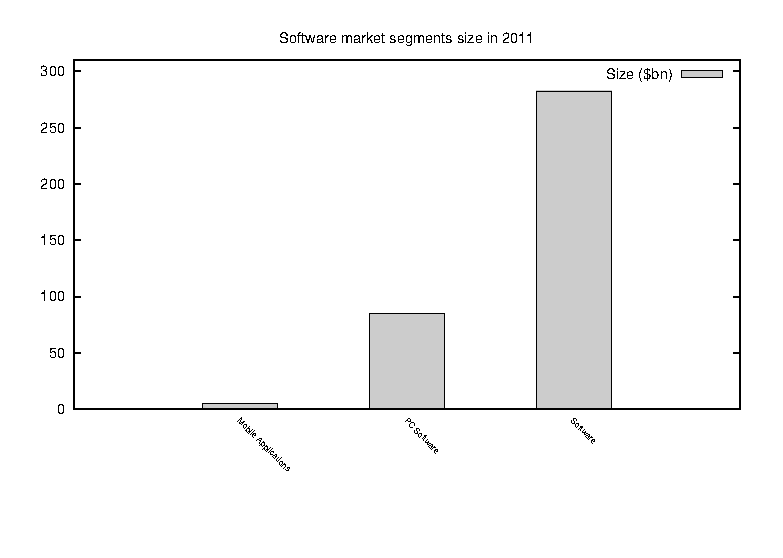
\includegraphics[width=1.0\textwidth]{markets}
\end{figure}

A main challenge for mobile app developers is producing and maintaining cross-platform applications. Although there are already plenty of tools that address writing such applications (please, see Table ~\ref{tab:crossPlatformTools}), there are three main problems with them:

\begin{itemize}
\item
all of them require learning additional languages (e.g. HTML, JavaScript, or
Lua),
\item
most of them violate the Apple SDK Agreement \cite{P5} \cite{P6} by
producing apps originating from disallowed languages, and
\item
none of them can deal with automatic porting of already existing code that was
originally written for a specific platform.
\end{itemize}

\begin{table}
    \label{tab:crossPlatformTools}
    \caption{Comparison of popular cross-platform mobile tools \cite{P4}}
    \centering
    \begin{tabular}{ | l | p{4.4cm} | p{2.6cm} | p{3cm} |}
    \hline
    Name & Required Knowledge & Cost & Since \\ \hline
    Sencha Touch & HTML, CSS, JavaScript & Free & November 2010 \\ \hline
    jQuery Mobile & HTML, CSS, jQuery & Free & October 2010 \\ \hline
    Tiggzi & HTML, CSS, JavaScript & \$0 - \$180 pm & Unknown \\ \hline
    AppMakr & HTML, CSS & \$79 pm & January 2010 \\ \hline
    iBuildApp & HTML, CSS & \$10 pm & 2010 \\ \hline
    Widgetbox & HTML, CSS & \$25 - \$100 pm & October 2010 \\ \hline
    foneFrame & HTML, CSS, JavaScript & \$0 - \$59 & Unknown \\ \hline
    phoneGap & HTML, CSS, JavaScript & Free & August 2008 \\ \hline
    Corona & Lua & \$200 - \$350 py & December 2009 \\ \hline
    \end{tabular}
\end{table}

These points justify the creation of a compiler that can take the source code of
an iPhone application written in Objective-C and produce an equivalent Android
application. However, there are a couple of major issues with this idea:
firstly, the libraries used for iPhone development - Cocoa API - are proprietary
and thus can not be compiled for Android, and secondly, interface guidelines for
the two platforms differ and thus interfaces can not be literally translated.
Fortunately, there is a community effort to solve the first problem - the
GNUStep project. And while the interface guidelines differ, they are
specific enough to make the detection and translation of idioms possible.

This discussion outlines two of the three major components that a system of the required type must have: a version of the Cocoa API, compiled for the Android platform, and an interface translation module. The third necessary component is, of course, a compiler core that can translate the actual program logic. As building the whole system is an ambitious task for an honours project, it was decided that the effort would be concentrated on research on the program logic component.

\section{Goals}

As outlined in the background section, the goal of this project is to investigate the possibility of building a system, using which, an Objective-C code can be compiled to a Dalvik executable and can be ran on an Android emulator or an actual Android based smart phone. Essential properties of the system are:
\begin{itemize}
\item
correctness: the produced program should be working as described by the source code. More formally, for a given input the program should produce the same output as native programs compiled by the Gnu Compiler Collection (gcc) and clang+llvm, where the two agree;
\item
speed: the time to build a typical program should be acceptable (in the order of minutes at worst).
\end{itemize}

In addition to these, it is desirable that the resulting system has the following properties:

\begin{itemize}
\item
performance of produced code: the produced program should be reasonably fast (same order of magnitude), when compared to an identical program, written in Java and built using the standard tool chain (Android Development Kit);
\item
size of produced code: the size of the produced program should be reasonably small, when compared to an identical program, written in Java and built using the standard tool chain.
\end{itemize}

TODO: finish and link with conclusion

\section{Overview}

\chapter{Background}

\section{Objective-C}

Objective-C was originally developped between 1981 and 1983 by Brad Cox and Tom Love as a superset of the C programming language that was strongly inspired by Smalltalk and incorporates its object oriented model\cite{Biancuzzi2009}. The creators of the language concentrated on building an extension that relies on run-time libraries and dynamic binding to improve the ease of integration of different components, rather than inventing a complex powerful software manufacturing system from scratch, which is the approach taken with C++.

The Objective-C language implements the object-oriented paradigm in a different way than the more widely used and successful C++ language. The former's object oriented model is based on Smalltalk, as previously mentioned, while that part of the latter is modelled after the aproach taken in the Simula language. As a result of this, even though the two languages are good at tackling similar domains of problems, their core principles are different. Objective-C was designed with simplicity in mind - the language architects aimed at adding the absolute minimum of additional features that would enable the programmers to write object-oriented programs. Backward compatibility with C and understandability were also main objectives of the project. In contrast, Bjarne Stroutstrup (the creator of C++) wanted to create a language for maximum efficiency that allowed him and fellow collegues to "express program organisation as could be done in Simula"\cite{Biancuzzi2009}. The focus was on power and speed, and as a result C++ turned out to be more complex and harder to understand than Objective-C. However, in the long run it also turned out to be more popular, the reason for which the Objective-C creators find in the fact that C++ was given away for free by AT\&T, rather than in actual benefits of the language. The compiler and support libraries of Objective-C were the only revenue sources of Stepstone (the company of Love and Cox), so they couldn't afford to open source the project, and thus it remained mostly unpopular.

The first notable recognition of the language was when it was chosen as the native language for the NeXTStep 1.0 operating system in 1989 - the first mature operating system of NeXT Computer. It is hard to find the reasons for choosing Objective-C over C++ in that setting. A propaganda NeXTStep manual from 1992\cite{NeXTCorporation1991} claims that NeXT chose Objective-C for its ease of learning and because of its support for dynamic binding, arguing that the latter allows for more seemless updates of the system, but this can be achieved equally easy by using shared/dynamically linked libraries. The author speculates that a major part of the decision was the need to differentiate from other OS vendors of the time and create a NeXT specific developer community and user base. Whatever the reason, the result remains and it is a popularisation of the Objective-C language.

NeXT later acquired the rights over Objective-C in 1995 and became the main advocator of the language. The company itself was acquired by Apple Inc. in 1997 and the NeXTStep operating system eventually evolved into what became known as Mac OS X over the period of four years. This way Objective-C propagated its way into the Mac computers of today. Native Mac apps are developed using the proprietary Cocoa API, which is written in Objective-C. A mobile version of this API - Cocoa Touch - is what is used for developing applications for the iPhone, iPod, and iPad.

Since programming in the past couple of decades has not been restricted to a selected few, but rather an essential skill sometimes compared to literacy in its importance, NeXT/Apple have recognised that they need to provide the general public (rather than only Mac users) with tools that allow creation of Objective-C programs if they want to make Objective-C a competative and popular language.

The first such initiative was OpenStep which was an object-oriented API for non-NeXTStep operating systems. The GNUStep project is an open source implementation of Cocoa that is based on OpenStep. Later, a team of NeXT/Apple engineers, lead by Steve Naroff developed the GCC Objective-C frontend. However, it relied on run-time libraries, which were not open sourced, so this effort remained useless to the general public. Finally, Apple invested in building the Objective-C frontend to Clang in 2007, which enabled the author to undertake this project.

Thanks to the existence of Clang, the reader need not understand the minute details of the Objective-C language as it is translated by this LLVM frontend to LLVM bytecode.

\section{LLVM and Clang}

\subsection{History}

LLVM was initially concieved as "a compilation strategy" that was designed to provide "effective multi-stage optimisation and more effective profile-driven optimisation, and to do so without changes to the traditional build process or programmer intervention"\cite{Lattner2002}. It was started as the Masters Thesis project of Chris Lattner under the supervision of Professor Vikram Adve in the year of 2000 at the University of Illinois at Urbana-Champaign. The main goals were to lay the foundation of a modern modular compiler, that has similar interface to its contemporaries and predecessors. The paper was published in 2003, and the LLVM infrastructure was open sourced, subsequently being widely adopted by the community and researchers\cite{Lattner}. In 2005, Apple hired Lattner to work at their compilation team and during the following seven years he advanced in positions to reach that of "Director and Architect, Developer Tools Department" in January 2013. Now he is responsible for the management of the entire Developer Tools department at Apple[cite http://www.nondot.org/sabre/Resume.html]. Apart from an example of impressive personal development, this is important for the evolution of LLVM, as during his career at Apple Lattner has mainly been working on LLVM and related tools, including Clang.

\subsection{Structure}

There are four stages of compilation included in LLVM: pre-linking compilation, link-time optimisations, run-time optimisations, and offline optimisations\cite{Lattner2002}. The first two stages are common in traditional compilers and include static analysis and classical optimisations. After stage two, the program is compiled to machine code, but high-level type information is also included in the output. This is one of the key novelties in LLVM, as this information is later used to perform the run-time optimisations and offline optimisations.

During execution of an LLVM compiled program, profile information is gathered from the usage statistics. This is different to the usual approach of profiling, as the usage information is actual, user specific data, rather than synthetic data that is fabricated by the developer. This way, the pitfall of profiling for the wrong data is avoided and the increase of performance is higher. In addition to this, the whole profiling process is automated and the overhead of effort is removed. 

Other activities that take place during execution of the program are run-time optimisations. These are optimisations that can be found in standard Just-In-Time (JIT) compilers, but also optimisations that use the profiling data to make common cases in the code faster, for the price of slowing down less common control flow paths. If there are profile driven optimisations that are too expensive to perform, they are sheduled for the offline optimiser.

The offline optimisations in LLVM are more aggressive dynamic optimisations that are too expensive to run alongisde the program, so they are performed when the system is idle. They are particularly useful for programs in which the majority of time of the execution is spent over a large part of the code, rather than having a particular "hot" spot. In such cases the profiler would detect optimisation opportunities, but it would not be beneficial to actually perform them in run-time, so they are delayed to when the offline optimiser can step in.

\subsection{Language}

The instruction set that LLVM uses provides an infinite amount of typed virtual registers in Static Single Assignment (SSA) form, which hold values of primitive types. The primitive types include integers, floating point numbers, and pointers. 

Memory is accessed via the store and load operations and is partitioned in global area, stack, and heap. Stack variables are allocated using the alloca instruction and are freed automatically when the function returns. Heap variables are allocated using malloc and need to be freed explicitly using the free instruction. In this way, the memory management in the LLVM language is similar to the C programming language.

The arithmetic and logical operations are in three-address form. The available arithmetic operations are: add, sub, mul, div, and rem. The names are self explanatory and correspond to the usual operations in arithmetic. Div and rem are whole number division and remainder functions. The available logical operations are: not, and, or, xor, shl, and shr. Additionally there is a collection of comparison instructions that produces a boolean result: seteq, setne, setlt, setgt, setle, and setge. Respectively, they stand for: equal, not equal, less than, greater than, less than or equal, and greater than or equal. Other instructions can take 0, 3, or a variable number of arguments. Examples are the call instructions and the SSA phi instruction.

All instructions in the LLVM instruction set are polymorphic. This means that they can operate on different types and do not need to have special versions for each of the possible types. The types of the operands also define the semantics of the instruction.

\subsection{Building a new backend}

Because of the high modularity of the architecture of LLVM it is possible to build new backends and plug them in the whole system. A backend is basically a module that takes the LLVM internal representation and translates the program to a specific target native code. Since Clang includes an Objective-C frontend for LLVM, the author concentrated on developing only a backend that produces Dalvik bytecode from LLVM internal representation.

There are different ways to do this, depending on the amount of the recommended structure that the developer wants to incorporate in the backend. Ideally, it should extend a large number of LLVM classes and provide target specific details\cite{P8}. This way more of the previously discussed LLVM features can be enabled. However, if the aim is simply to get a working prototype, it is sufficient to extend only one class (see section Implementation) and then to register the backend.

Also, work in LLVM is done in passes of different modularity (block, function, or module), and the developer that is extending the functionality can decide which one (or more) of those they want to implement. However, when writing a backend it is obvoius that the whole program needs to be processed, so writing a module (the largest granularity) pass is sufficient.

For example, if one wishes to create a new target called Blank, they must create a new subdirectory in llvm/lib/Target with the name of the target (Blank). That folder will contain the new backend implementation. This folder contains classes for different modules of the backend, e.g. a module for parsing assembly, one for JIT compilation, one for   

\section{Android and Dalvik}

\subsection{Android}

Android was revealed on the 5th November 2007 by Google, when they introduced the Open Handset Alliance (OHA)\cite{DeLacey2007}. The alliance comprises of several dozens of telecommunication companies and their aim is to produce more open and customisable mobile phones. The major product to achieve this is Android - an open source mobile operating system based on Linux.

Historically, the development of the Android operating system starts around 2003 at a company called Android Inc\cite{BloombergBusinessweek2005}. The project is developed under high secrecy and little is known about its existence before it was introduced in 2007, apart from the fact that the company engaged with it was acquired by Google in 2005.

Android entered a market that was dominated by conservative vendors: Apple, Microsoft, and RIM. Their philosophies don't reserve a place for the idea of open-source software and this is what was different about the new operating system. During the following five years the community of programmers developing Android apps grew rapidly, producing around 700 000 apps for the platform\cite{Islam2012}. Today Android is the most popular mobile operating system, owning three quarters of the market share\cite{IDC2012}.

In addition to advocating open-source, Android has the advantage that it allows hardware manufactures to concentrate on improving the devices and not worry about the software that runs on them. This way it is very useful for new companies that don't have the financial or technical resource to develop their own operating system. As a result, Android is even employed in devices it was not originally intended for, like TV sets and game consoles\cite{Telecompaper2012}\cite{Etherington2013}.

\subsection{Dalvik}

Dalvik is the virtual machine (VM) that runs on Android devices. Since Android applications are written in Java, Dalvik is similar to a Java Virtual Machine (JVM), but has several key differences.

First of all, Dalvik is register based, compared to the stack based JVM. This means that arguments for the instructions reside in virtual registers (a total of 65K of them) and not on a stack. Thus, the push and pop instructions that are used to manipulate the stack in order to execute stack based operations can be removed, resulting in less instructions, and thus smaller programs - important improvement for mobile applications.

Secondly, Dalvik does not use the defaut Java GUI frameworks (i.e. AWT or Swing) but rather relies on a dedicated one. However, open source frameworks have been successfully ported to run on Android, notably the popular Qt framework, so it is still possible to write applications which are independent of the VM  used.

Most importantly though, due to the subtle differences between the Dalvik bytecode and the Java bytecode, Dalvik has its own file format - .dex. The .dex files are usually compiled from JAVA .class files using the dx tool from the Android SDK. However, the different file format further distantiates the two virtual machines and makes them incompatible in the strict sense.

\subsection{Smali}

Smali is an assembler for the dex format, the syntax for which is loosly based on Jasmin's syntax - an assembly code for Java\cite{GoogleProjectHosting2013}.

Smali code, although being assembly code for a virtual machine, shares a lot with real RISC architectures. Arithmetic and logical operations are in three-address mode\cite{TheAndroidOpenSourceProject2007} which is the same as LLVM's. An important thing to note is that there are no boolean comparison operators. In order to compare numbers one has to use either the ternary comparison operators (returning -1, 0, or 1 respectively for less than, equal, or greater than results) that can not take short (single word) integer values, or the family of conditional branches if-eq, if-ne, if-lt, if-gt, if-le, and if-ge. The difference of the two approaches is examined in the implementation section.

Another dissimilarity from LLVM's internal representation is that arithmetic and logical operations in smali are not polymorphic, e.g. there are four versions of add: add-int, add-long, add-float, and add-double. There are also versions for when one of the operands is a literal, and versions taking only two registers. This flexibility allows for selecting the minimum amount of instructions in each context and thus achieving the desired reduction of program size.

Finally, there are two other operation classes relevant to this project: move and const. There are 13 variants of move, each specific for a different situation, and the behaviour is generally moving the contents of one register to another. The variants of const are 11, and they are intended to move different kinds of literal values to a register.

\chapter{Design and Implementation}

\section{Design}

Before the commencing of the work on the project, it was agreed that the best approach is to base the system on the LLVM compiler infrastructure. There are multiple advantages that come with building upon LLVM:
\begin{itemize}
\item
Firstly, LLVM comes with clang - a complete frontend for languages based on the C programming language. This includes Objective-C, so basing Objective-Droid on LLVM would remove the need of producing front-end components like a parser or a lexer.
\item
Secondly, LLVM comes with a powerful middle end that contains a wide range of optimizations \cite{P7}. Including them in Objective-Droid would be highly beneficial to the quality of the output, while at the same time, it would be infeasible and unnecessary to duplicate all the work of implementing these optimizations.
\item
Thirdly, using an established compiler infrastructure as a foundation would provide an interface that developers are already used to, at no additional effort. This would reduce the learning curve for users of Objective-Droid and let them feel more confident about using the tool.
\item
Fourthly, building a backend for LLVM by the guidelines would allow it to be contributed to the project, thus all, or parts of Objective-Droid can be given back to the compiler developer community easier than if it is being developed from scratch.
\end{itemize}
Thus, the first essential component of the Objective-Droid system is the LLVM backend. The target code was decided to be smali code, as there are already assembling tools for it that produce Dalvik binaries.

The second essential component is a packager that given the smali code assembles it, packages it, and signs the package. This would allow the package to be installed and tested on an emulator or a phone.

The final component of the Objective-Droid system is a wrapper program or a script that automates the whole process of compiling, packaging, and possibly installing the program on a phone. This script would be useful for testing, but is not mandatory.

For a summary of the design, please see Figure ~\ref{fig:design}.

\begin{figure}[htp]
  \label{fig:design}
  \caption{Overall design of the Objective-Droid system.}
  \centering
    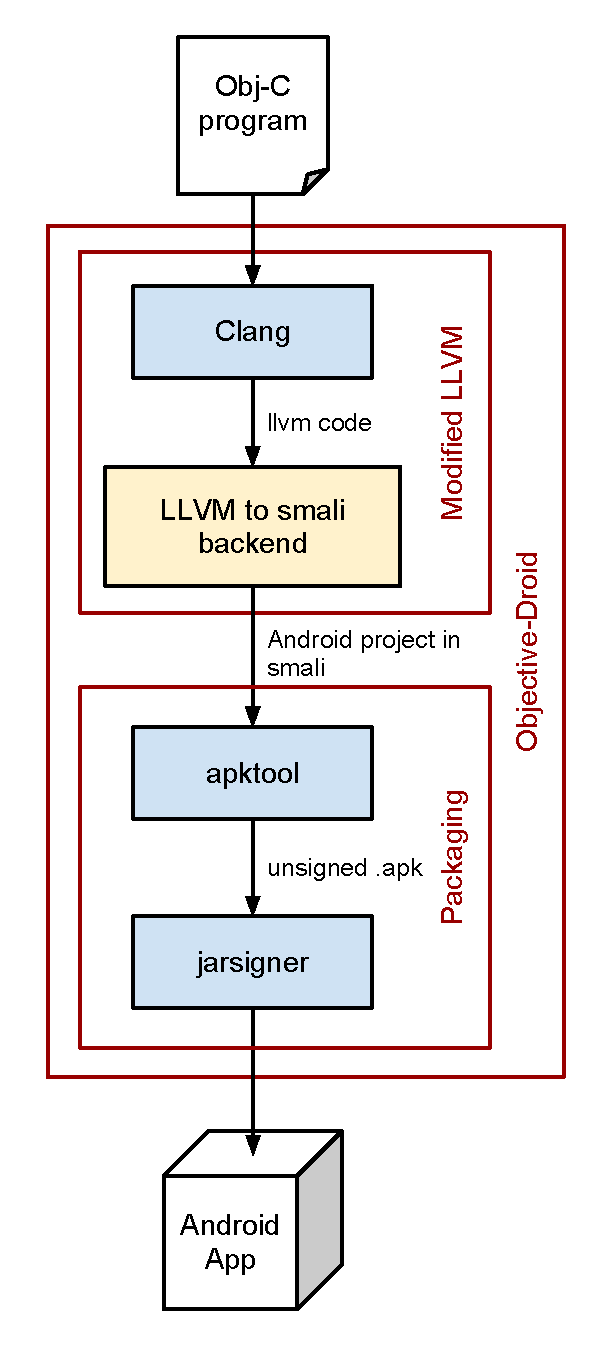
\includegraphics[width=0.6\textwidth]{design}
\end{figure}

\section{Implementation}

\subsection{File structure}

As apparent from the design outline, the most integral part of the project is building the LLVM backend. This required familiarising with the conventions that are accepted within the LLVM community for undertaking such work, and understanding the general structure of a backend.

An LLVM backend needs to be implemented as a subclass of the TargetMachine class \cite{P8}. Depending on the features of the target architecture, the implementation needs to provide a suite of files. E.g. if MIPS is the target architecture, the implementation needs to provide files that describe: the instructions, the registers, the interface for JIT compilation, etc. On the other hand, if the target is not a real architecture, but rather a high-level language, the implementation can be as simple as a single class. This is the case of the backend that produces C++ code.

The initial approach taken when developing the Objective-Droid backend was to follow the general structure and provide separate classes for the different functions of the backend. However, this was decided to be overly complicated, especially when compared to the approach of the C++ backend. It was argued that the code that the backend has to produce - smali code - is not actual machine code, so it does not need many of the classes that a code for a real architecture would require (e.g. an assembler definition).

Thus, for the main part of the project the backend was developed in a single monolithic class. Still, attempting to use the full target class hierarchy was not a waste of time, as it provided an insight of how the LLVM project works - an insight that was helpful later.

The decision to write the whole backend as a single class provoked the danger of bad maintainability. Thus, during development, effort was put towards writing simpler and cleaner code at first, and then optimising the common parts of it. Also, comments were put as documentation, as general comments, and as specific comments explaining complicated code. The overall result was readable code that is easy to understand for a newcomer to the project.

\subsection{{\tt Target} class}

The main class of the implementation inherits the {\tt ModulePass} class of LLVM. The {\tt ModulePass} is typically used for passes that manipulate the whole program, thus it serves the needs of the Objective-Droid backend. This makes the {\tt runOnModule} method to be the entry point of the class. This method is given a description of the program in a {\tt Module} object as an argument and returns {\tt false} on success.

The implementation of the {\tt runOnModule} method simply builds a corresponding Android {\tt Activity} class by iterating over the global variables and functions of the {\tt Module}, and translating them to static fields and to static methods, respectively. The boiler-plate code for the class includes a start up method - {\tt onCreate} - which is a standard way of starting up an Android {\tt Activity}. It invokes the translation of the main function of the supplied Objective-C code, and calls the typical {\tt finish} method that terminates the program.

The functions are translated by iterating over the instructions in them and translating each one in separately. It was found that for most instructions this is trivial, and others were either simply translated to a series of instructions (as in the case of comparison instructions) or emulated by a dedicated external library. This approach would result in a slightly lower performance of the output program, but ensures good performance of compilation and simplicity of the compiler.

\chapter{Related Work}

\section{LLJVM}

LLJVM is another project build on top of LLVM. The project was originally made available to the public around November 2009 [ref hacker news.], development died out about a year later [ref github], and is not maintained any more.

Its aim is (or rather - was) to provide a way of running C code on a Java Virtual Machine. The approach is quite similar to the one taken with Objective-Droid: source code is compiled to llvm bytecode, then it is ran through the LLJVM backend to produce Jasmin (assembly language for Java), and it is linked and assembled. Just as a remainder for the reader: in Objective-Droid Objective-C code is compiled to llvm bytecode, then translated by the backend to smali code, linked and assembled.

Unfortunatelly, the author could not build the LLJVM project from source, as it depends on a very specific LLVM version (2.7) which proved quite hard to build on the testing configuration of the time. Other attempts have revealed that the LLJVM code is not compatible with newer versions of LLVM, in particular 3.2. Furthermore, there is no compiled version available, and thus it could not be tested properly. However, from the web page of the project (and the positive comments on it) it appears that the project was at least partially successful.

\section{NestedVM}

Another C-to-Java compiler is NestedVM. In contrast with LLJVM, it relies on gcc, rather than on LLVM, and uses MIPS assembly code as intermediate representation \cite{AllietMegacz:ivme:2004}. It can also target the Java language, which makes it more flexible than LLJVM. According to the paper that introduces NestedVM, it is novel in not using native interfaces like JNI to produce Java bytecode from a C program.

NestedVM is an impressive effort, as it provides a runtime that implements a lot of mechanisms found in C programs that are not straightforward to translate to Java, including: unsigned numbers, file I/O, process-level memory management, and syscalls. There is an even more advanced runtime that emulates a large portion of the POSIX API, notably: maintaining filesystems and device nodes, multiprocessing, and simple networking support. Another interesting feature is that the 64KB limit on the size of Java methods is overcome by splitting long programs to multiple methods and linking them together (called trampoline transformation in the paper.)

The paper reports only three to ten times performance reduction when compared to native execution, and claims that this makes NativeVM an attractive solution for code which is not performance-critical.

Objective-Droid is not as complex as NestedVM, as the goal of the project is not to create a complete system, but rather a prototype that shows that it is possible to run Objective-C programs on Dalvik. For this reason many of the features available in NestedVM are not implemented in Objective-Droid, but it is still possible to compare their performance, as shown in the evaluation section.

\chapter{Evaluation}

\section{Correctness}

\section{Performance}

\chapter{Conclusions}

% use the following and \cite{} as above if you use bibtex
% otherwise generate bibtem entries
\bibliographystyle{plain}
\bibliography{final}

\end{document}